\section{比值的分布}
\label{sec:rvt-ratios}

两段独立的等待时间之比、一个测量误差除以另一个估计出来的尺度，都是比值$R=X/Y$。比值与乘积只差一个倒数，但分母可以很接近零，这时比值会非常大。这一节的主题是这种情况怎样影响比值的尾部与矩。

\paragraph{分母不能取零}
$R=X/Y$要有定义，首先需要$\mathbb{P}(Y=0)=0$。$(X,Y)$有联合密度时这自动成立；离散时要事先排除$Y$取零的情形，或者把它作为“比值无定义”的事件单独报告。

离散时仍用原像规则：$R=r$当且仅当$(X,Y)$落在直线$x=ry$上的格点之一。两枚骰子的比值$X_1/X_2=2$的原像是$\{(2,1),(4,2),(6,3)\}$，于是
\[
 \mathbb{P}\Bigl(\frac{X_1}{X_2}=2\Bigr)=\frac{3}{36}=\frac1{12},\qquad \mathbb{P}\Bigl(\frac{X_1}{X_2}=1\Bigr)=\frac{6}{36}=\frac16 .
\]

\paragraph{比值与分母的联合换元}
有密度时，取辅助坐标$W=Y$。映射$(x,y)\mapsto(r,w)=(x/y,y)$在$y\neq0$的区域上一一，逆映射是$x=rw$、$y=w$，Jacobian行列式为
\[
 \det\begin{pmatrix}w&r\\0&1\end{pmatrix}=w .
\]
由式~\eqref{eq:rvt-multivariate-density}得到$f_{R,W}(r,w)=f_{X,Y}(rw,w)\lvert w\rvert$，再积掉$w$，就得到下面的公式。

\begin{theorem}[比值的密度]
\label{thm:rvt-ratio-density}
设$(X,Y)$有联合密度$f_{X,Y}$，则$R=X/Y$有密度
\begin{equation}
 f_R(r)=\int_{\mathbb{R}}f_{X,Y}(rw,w)\,\lvert w\rvert\,\mathrm{d}w .
 \label{eq:rvt-ratio-density}
\end{equation}
若$X$与$Y$独立，被积函数中的$f_{X,Y}(rw,w)$换成$f_X(rw)\,f_Y(w)$。
\end{theorem}

与乘积公式中的$1/\lvert x\rvert$相反，这里的因子是$\lvert w\rvert$。固定分母$Y=w$，$R$落在$[r,r+\Delta r]$等价于$X$落在长度为$\lvert w\rvert\Delta r$的区间里；分母越小，同样一段$\Delta r$对应的$X$区间越短。所以分母接近零的样本并不集中在某个$r$附近，而是散到很大的$\lvert r\rvert$上去。

\paragraph{均匀变量之比}
设$U,V$独立且都服从$\operatorname{Unif}(0,1)$，$R=U/V$取值于$(0,\infty)$。代入式~\eqref{eq:rvt-ratio-density}，被积函数非零要求$0<w<1$且$0<rw<1$，即$0<w<\min(1,1/r)$，于是
\[
 f_R(r)=\int_0^{\min(1,1/r)}w\,\mathrm{d}w=
 \begin{cases}
  1/2, & 0<r\leq1,\\
  1/(2r^2), & r>1 .
 \end{cases}
\]

在单位正方形里直接看原像也能得到它。$U/V\leq r$即$u\leq rv$，是直线$u=rv$下方的部分：$r\leq1$时是面积为$r/2$的三角形，$r>1$时是正方形去掉面积为$1/(2r)$的三角形。于是
\[
 F_R(r)=
 \begin{cases}
  r/2, & 0<r\leq1,\\
  1-1/(2r), & r>1 .
 \end{cases}
\]
$F_R(1)=1/2$，与$U,V$对称一致。

尾概率$\mathbb{P}(R>r)=1/(2r)$衰减得很慢，均值不存在：
\[
 \mathbb{E}[R]\geq\int_1^\infty r\cdot\frac{1}{2r^2}\,\mathrm{d}r=\infty .
\]
用独立性也能看出这一点：$\mathbb{E}[U/V]=\mathbb{E}[U]\,\mathbb{E}[1/V]$，而$\mathbb{E}[1/V]=\int_0^1v^{-1}\,\mathrm{d}v$发散。分子与分母都有界，比值的均值却是无穷，原因全在分母靠近零的那一小块：$V<\varepsilon$的概率是$\varepsilon$，而在这个事件上$R>U/\varepsilon$。

\paragraph{独立标准高斯之比}
设$X,Y$独立且都服从$\mathcal{N}(0,1)$。由式~\eqref{eq:rvt-ratio-density}，两个高斯密度的乘积给出指数$-(r^2w^2+w^2)/2$；被积函数关于$w$是偶函数，只算$w>0$再乘$2$，得到
\begin{equation}
 f_R(r)=\frac{2}{2\pi}\int_0^\infty w\,\mathrm{e}^{-(1+r^2)w^2/2}\,\mathrm{d}w=\frac{1}{\pi(1+r^2)},\qquad r\in\mathbb{R} .
 \label{eq:rvt-cauchy}
\end{equation}
这是第~\ref{chap:common-distributions}章的Cauchy分布，即自由度为$1$的t分布。

几何上看得更清楚。由式~\eqref{eq:rvt-polar-density}，$(X,Y)$的方向角$\Theta$服从均匀分布，且与半径独立；比值$Y/X=\tan\Theta$只取决于方向，与半径无关。$\tan$以$\pi$为周期，所以$\Theta$只需看作$(-\pi/2,\pi/2)$上的均匀变量，于是
\[
 \mathbb{P}\Bigl(\frac YX\leq t\Bigr)=\frac{\arctan t+\pi/2}{\pi} ,
\]
求导就是式~\eqref{eq:rvt-cauchy}。由对称性$X/Y$与$Y/X$同分布。这个论证只用了方向均匀，所以任何联合密度只依赖于$x^2+y^2$的$(X,Y)$，比值都是Cauchy分布。

图~\ref{fig:rvt-ratio-uniform}(c)中，$Y/X\leq1$的原像是两个对顶的扇形，张角合计$3\pi/2$，占整个圆周的$3/4$，所以$\mathbb{P}(Y/X\leq1)=3/4$，与上式在$t=1$处的值一致。

\begin{BookInlineFigure}
  \centering
  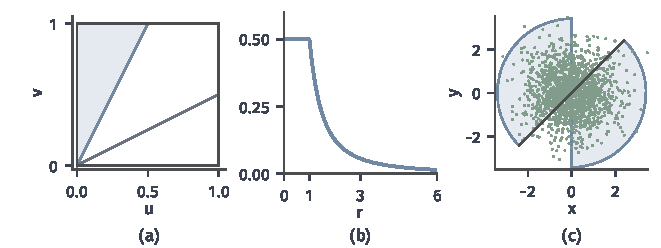
\includegraphics[width=112mm]{figures/07-probability/01-elementary-probability/matplotlib/rvt-ratio-uniform/figure.pdf}
  \caption{比值的原像。(a)$U,V\sim\operatorname{Unif}(0,1)$独立，浅蓝区域是$U/V\leq0.5$的原像，面积$1/4$；灰线是$U/V=2$。(b)$U/V$的密度（蓝），$r>1$后按$1/(2r^2)$衰减。(c)独立标准高斯，浅蓝的两个对顶扇形是$Y/X\leq1$的原像，绿点是$1500$个模拟样本（种子$17$）。}
  \label{fig:rvt-ratio-uniform}
\end{BookInlineFigure}

Cauchy分布的尾部是
\[
 \mathbb{P}(\lvert R\rvert>t)=1-\frac2\pi\arctan t\approx\frac{2}{\pi t},\qquad t\to\infty ,
\]
被积函数$\lvert r\rvert/(\pi(1+r^2))$在远处像$1/(\pi\lvert r\rvert)$，积分像$\int\mathrm{d}r/r$一样发散，所以$\mathbb{E}\lvert R\rvert=\infty$，均值不存在。机制与均匀比值相同：$\lvert Y\rvert<\varepsilon$的概率约为$2\varepsilon\varphi(0)\approx0.80\varepsilon$，在这个事件上$\lvert R\rvert>\lvert X\rvert/\varepsilon$。分母落在零附近的概率与$\varepsilon$成正比，比值超过$1/\varepsilon$量级的概率也就与$\varepsilon$成正比，这正是$1/t$的尾部。

\paragraph{t分布的构造}
把分母换成一个不容易接近零的量，尾部就会变轻。设$Z\sim\mathcal{N}(0,1)$与$U\sim\chi^2_\nu$独立，$\nu>0$，定义
\begin{equation}
 T=\frac{Z}{\sqrt{U/\nu}} .
 \label{eq:rvt-t-construction}
\end{equation}
$\nu$为正整数时，由式~\eqref{eq:rvt-chi2-sum}，$U$可以看成$\nu$个独立标准高斯的平方和，$U/\nu$是它们的平均平方，分母是一个“估计出来的尺度”。下面分两步求$T$的密度。

第一步求分母$W=\sqrt{U/\nu}$的密度。$U$的密度是$\operatorname{Gamma}(\nu/2,1/2)$：
\[
 f_U(u)=\frac{u^{\nu/2-1}\mathrm{e}^{-u/2}}{2^{\nu/2}\Gamma(\nu/2)},\qquad u>0 .
\]
$w\mapsto u=\nu w^2$在$(0,\infty)$上递增，$\mathrm{d}u/\mathrm{d}w=2\nu w$。由式~\eqref{eq:rvt-monotone-density}，
\[
 f_W(w)=f_U(\nu w^2)\cdot2\nu w=\frac{2\,\nu^{\nu/2}}{2^{\nu/2}\Gamma(\nu/2)}\,w^{\nu-1}\mathrm{e}^{-\nu w^2/2},\qquad w>0 .
\]

第二步用比值公式。$Z$与$W$独立（定理~\ref{thm:rvt-group-independence}），由式~\eqref{eq:rvt-ratio-density}，
\[
 f_T(t)=\int_0^\infty\varphi(tw)\,f_W(w)\,w\,\mathrm{d}w=C_\nu\int_0^\infty w^{\nu}\mathrm{e}^{-(\nu+t^2)w^2/2}\,\mathrm{d}w ,
\]
其中常数是
\[
 C_\nu=\frac{2\,\nu^{\nu/2}}{\sqrt{2\pi}\,2^{\nu/2}\Gamma(\nu/2)} .
\]

剩下的积分作代换$s=(\nu+t^2)w^2/2$，化为Gamma积分：
\[
 \int_0^\infty w^{\nu}\mathrm{e}^{-(\nu+t^2)w^2/2}\,\mathrm{d}w=\frac12\Bigl(\frac{2}{\nu+t^2}\Bigr)^{(\nu+1)/2}\Gamma\Bigl(\frac{\nu+1}{2}\Bigr) .
\]
与$C_\nu$相乘时$2$的幂次恰好抵消，再把$(\nu+t^2)^{-(\nu+1)/2}$写成$\nu^{-(\nu+1)/2}(1+t^2/\nu)^{-(\nu+1)/2}$，得到
\begin{equation}
 f_T(t)=\frac{\Gamma\bigl((\nu+1)/2\bigr)}{\sqrt{\nu\pi}\,\Gamma(\nu/2)}\Bigl(1+\frac{t^2}{\nu}\Bigr)^{-(\nu+1)/2},\qquad t\in\mathbb{R} .
 \label{eq:rvt-t-density}
\end{equation}
这就是第~\ref{chap:common-distributions}章位置为$0$、尺度为$1$的t密度，式~\eqref{eq:rvt-t-construction}给出了它的来历。$\nu=1$时常数为$\Gamma(1)/(\sqrt\pi\,\Gamma(1/2))=1/\pi$，回到Cauchy分布；这与前面一致，因为$\chi^2_1$变量的平方根与$\lvert Y\rvert$同分布，而$Z/\lvert Y\rvert$与$Z/Y$同分布。

\paragraph{分母与矩}
$T$的哪些矩存在，由分母靠近零的概率决定。$Z$与$U$独立，对$k>0$，
\[
 \mathbb{E}\lvert T\rvert^{k}=\nu^{k/2}\,\mathbb{E}\lvert Z\rvert^{k}\,\mathbb{E}\bigl[U^{-k/2}\bigr] .
\]
$\mathbb{E}\lvert Z\rvert^{k}$总是有限的，问题在最后一个因子。$u\to0$时$f_U(u)$与$u^{\nu/2-1}$同阶，于是被积函数$u^{-k/2}f_U(u)$与$u^{(\nu-k)/2-1}$同阶；它在$0$附近可积当且仅当$(\nu-k)/2>0$，在无穷远处有指数衰减。所以
\begin{equation}
 \mathbb{E}\lvert T\rvert^{k}<\infty\iff k<\nu .
 \label{eq:rvt-t-moments}
\end{equation}

于是$\nu>1$时均值存在且为$0$，$\nu>2$时方差存在。$\nu>2$时把$u^{-1}f_U(u)$的积分写成Gamma积分，并用$\Gamma(\nu/2)=(\nu/2-1)\Gamma(\nu/2-1)$，得到
\[
 \mathbb{E}[1/U]=\frac{2^{\nu/2-1}\Gamma(\nu/2-1)}{2^{\nu/2}\Gamma(\nu/2)}=\frac{1}{\nu-2} .
\]
于是
\[
 \operatorname{Var}(T)=\nu\,\mathbb{E}[Z^2]\,\mathbb{E}[1/U]=\frac{\nu}{\nu-2} .
\]
与第~\ref{chap:common-distributions}章所列的t分布矩条件一致。尾部的阶数也由同一个机制决定：分母小于$\varepsilon$的概率与$\varepsilon^{\nu}$同阶，$\lvert T\rvert$超过$t$的概率就与$t^{-\nu}$同阶。

$\nu$增大时，$U/\nu$的均值为$1$、方差为$2/\nu$，分母越来越稳定地接近$1$，$T$越来越像$Z$。式~\eqref{eq:rvt-t-density}中的因子$(1+t^2/\nu)^{-(\nu+1)/2}$逐点趋于$\mathrm{e}^{-t^2/2}$，常数因子由Gamma函数的渐近式趋于$1/\sqrt{2\pi}$。图~\ref{fig:rvt-cauchy-t}比较$\nu=1$、$\nu=3$与高斯的密度和尾部。

\begin{BookInlineFigure}
  \centering
  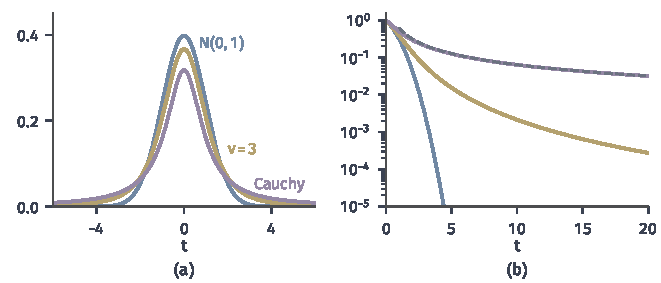
\includegraphics[width=112mm]{figures/07-probability/01-elementary-probability/matplotlib/rvt-cauchy-t/figure.pdf}
  \caption{比值分布的尾部。(a)标准高斯（蓝）、$\nu=3$的t分布（黄）与Cauchy分布（紫）的密度。(b)双侧尾概率$\mathbb{P}(\lvert T\rvert>t)$，纵轴为对数：高斯尾部（蓝）迅速下降，t分布（黄）与Cauchy分布（紫）分别按$t^{-3}$与$t^{-1}$的阶衰减，灰色虚线为$2/(\pi t)$。}
  \label{fig:rvt-cauchy-t}
\end{BookInlineFigure}
